\section{Pattern Matching and Image Recognition Algorithms}

  This section contains information on the pattern matching and image recognition algorithms that could utilised in the solution in order to help individuals devise a strategy for which data linked with them could be used for.

  \subsection{Pattern Matching}

    \subsubsection{Description}

      The bitap algorithm is an approximate or exact string matching algorithm that is one of the underlying algorithms of the UNIX ``agrep'' utility~\cite{}. It determines whether a given text contains a substring which is equal to a given pattern, where approximate equality is defined in terms of the Levenshtein distance – a complementary algorithm which determines how many changes must be made to a string or phrase in order to turn it into another string or phrase~\cite{}. In comparison to other algorithms, bitap does most of the work with bitwise operations, thus making it run super-fast.
      %This algorithm's library is available at https://code.google.com/p/google-diff-match-patch/.

      \begin{figure}
        \centering
        \begin{minipage}{14cm}
          \centering
          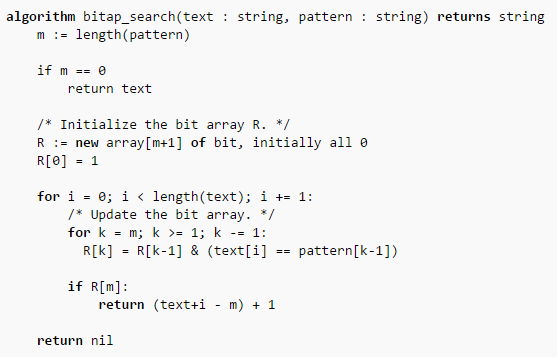
\includegraphics[width=14cm]{inc/bitap_algorithm.png}
          \caption{Bitap Algorithm Pseudocode}
          \label{fig:bitap_algorithm_pseudocode}
        \end{minipage}
      \end{figure}

    \subsubsection{Application}

      The solution will require access to two predefined datasets for classifying the information returned by search engine. The first dataset contains some sensitive keywords that will make a significant influence on public impression, such as drug abuse or achievement. The other dataset stores the words with a neutral, negative or positive emotion, and each word has a corresponding score, for example: disappointment with score -5, humiliation with score -8, honour with score +8 and success with score +6. 

      The steps for implementing this algorithm are as follows:
      \begin{enumerate}
        \item Search website articles for sensitive keywords and their relative location
        \item Search for ``emotional words'' that appear within the spatial locality of the sensitive keyword
        \item Calculate the score of the article or website based on the number of emotional words found
      \end{enumerate}

  \subsection{Image Recognition}

    \subsubsection{Description}

      Affine scale-invariant feature transform (or ASIFT) is computer vision algorithm that is used to detect and describe local features in images. It is regarded as an efficient method for determining matches between two arbitrarily-selected points within two widely separated views. Moreover, ASIFT is capable of finding a correspondence, even for pixels within an area with certain uniform properties, such as similar colours and textures~\cite{}.

      \begin{figure}
        \centering
        \begin{minipage}{14cm}
          \centering
          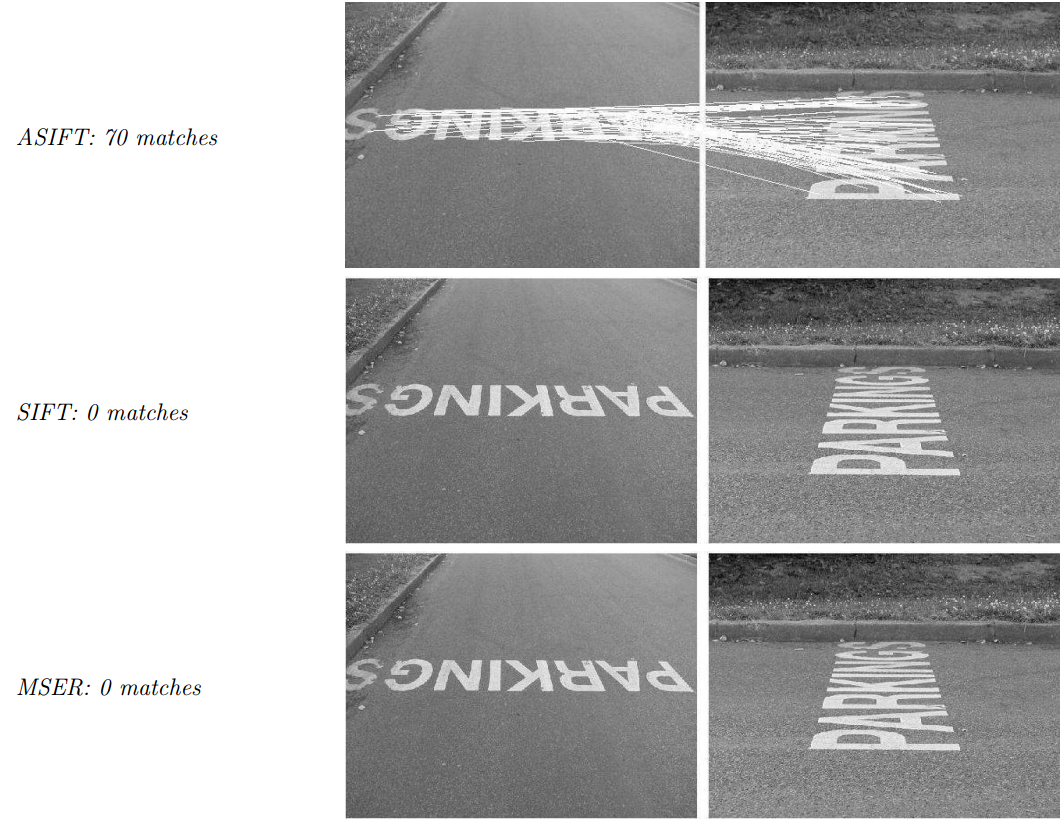
\includegraphics[width=14cm]{inc/image_recognition_comparison.png}
          \caption{Comparison of Image Recognition Algorithms}
          \label{fig:image_recognition_comparison}
        \end{minipage}
      \end{figure}

    \subsubsection{Application}

      During the text processing stage, a pattern matching algorithm can attempt to detect the purpose of an article or website. If it is determined that the page is an advertisement, then the image and face recognition algorithm can attempt to match the image with the relevant person's face. Once matched, a check can be carried out to determine whether or not the website has the right to use the portraiture.
